\documentclass{beamer}
\usetheme{Madrid}
\usecolortheme{default}
\usepackage{amsmath,amssymb,lmodern}
\usepackage{caption}
\usepackage{animate}
\usepackage{subcaption}
\usepackage{graphicx} %Loading the package
\graphicspath{{figures/}} %Setting the graphicspath
\title[Machine Learning]
{Treinamento de Machine Learning e Deep Learning}

\subtitle{Do Básico ao Avançado}

\author[Mafalda, Salomão] % (optional, for multiple authors)
{Salomão Machado Mafalda\inst{1}}

\institute[PAVIC] % (optional)
{
  \inst{1}%
  Universidade Federal do Acre\\
  PAVIC

}

\date[2023] % (optional)
{2023}

\logo{
\includegraphics[height=0.8cm]{ente}}

\definecolor{uoftblue}{RGB}{6,41,88}
\setbeamercolor{titlelike}{bg=uoftblue}
\setbeamerfont{title}{series=\bfseries}

\begin{document}

\frame{\titlepage}

\begin{frame}
\frametitle{Agenda}
\tableofcontents
\end{frame}



%==========================================================================================
\section{Perceptron}

\begin{frame}
	\frametitle{Perceptron}
	\begin{figure}
		\centering
		\label{fig:neuron}
		\includegraphics[width=0.4\linewidth]{neuron}
		\caption{Neurônio humano}
	\end{figure}
\end{frame}


%==========================================================================================
\begin{frame}
	\frametitle{Perceptron}
	\begin{figure}
		\centering
		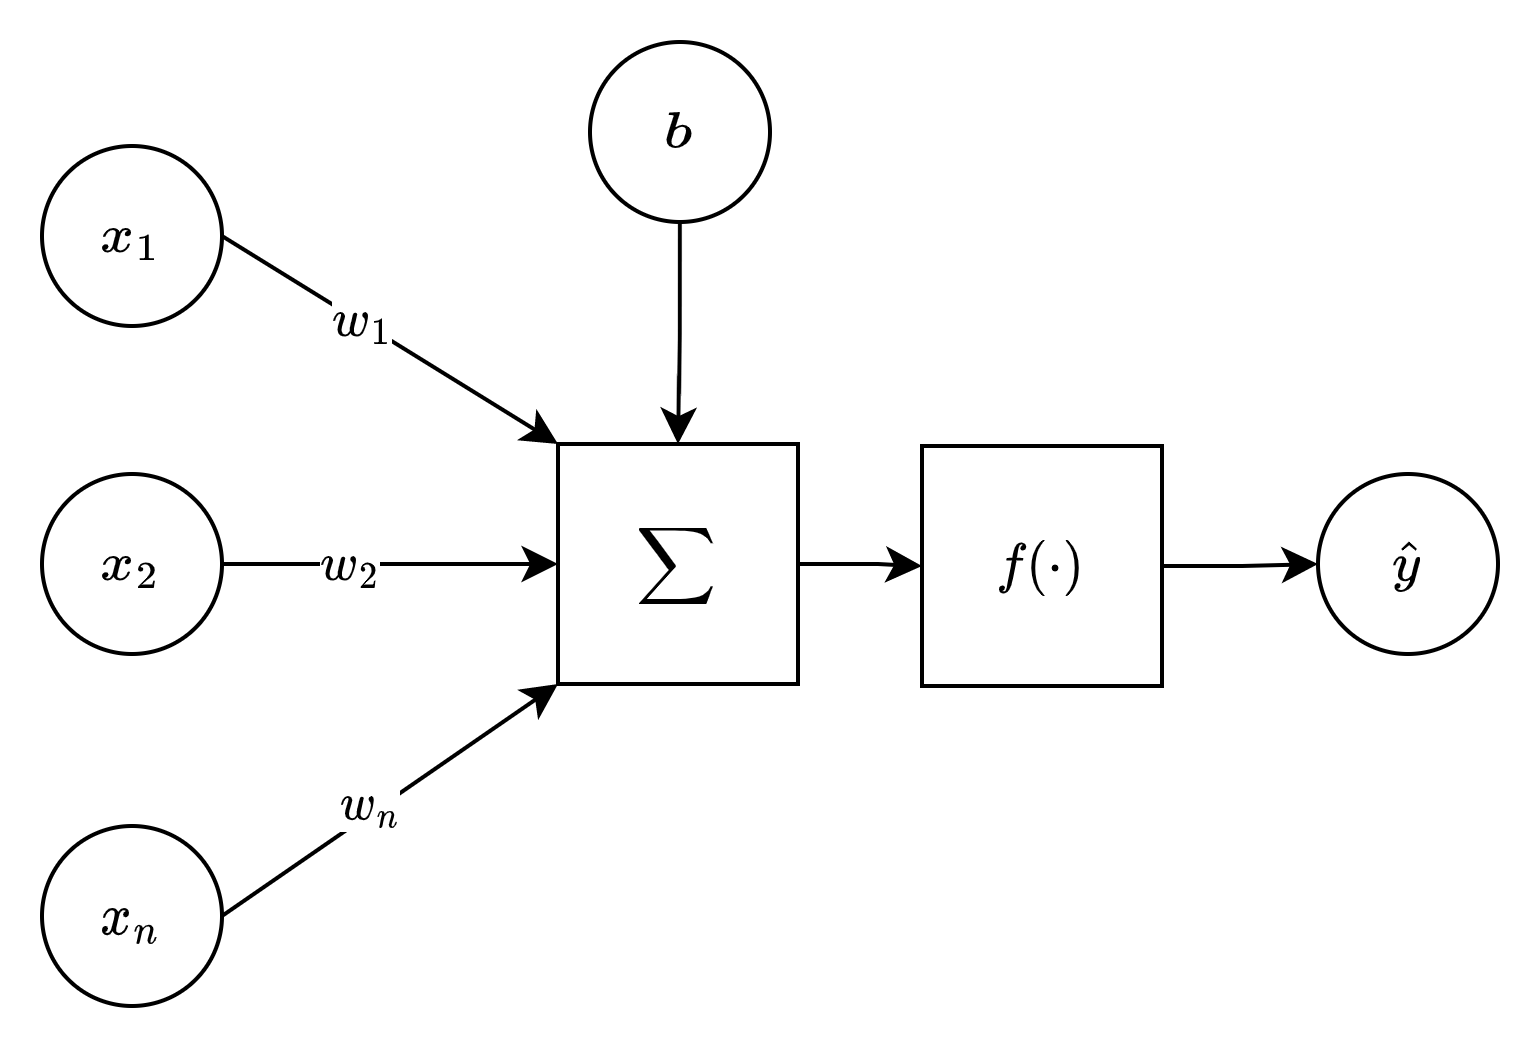
\includegraphics[width=0.4\linewidth]{figures/neuron_ai}
		\caption{Neurônio Artificial}
		\label{fig:neuronai}
	\end{figure}
\end{frame}

%==========================================================================================
\begin{frame}
	\frametitle{Perceptron}
	\begin{figure}
		\centering
		\begin{subfigure}{.45\textwidth}
			\includegraphics[width=1\linewidth]{figures/neuron}
			\caption{Neurônio Humano}
		\end{subfigure}
		\begin{subfigure}{.45\textwidth}
			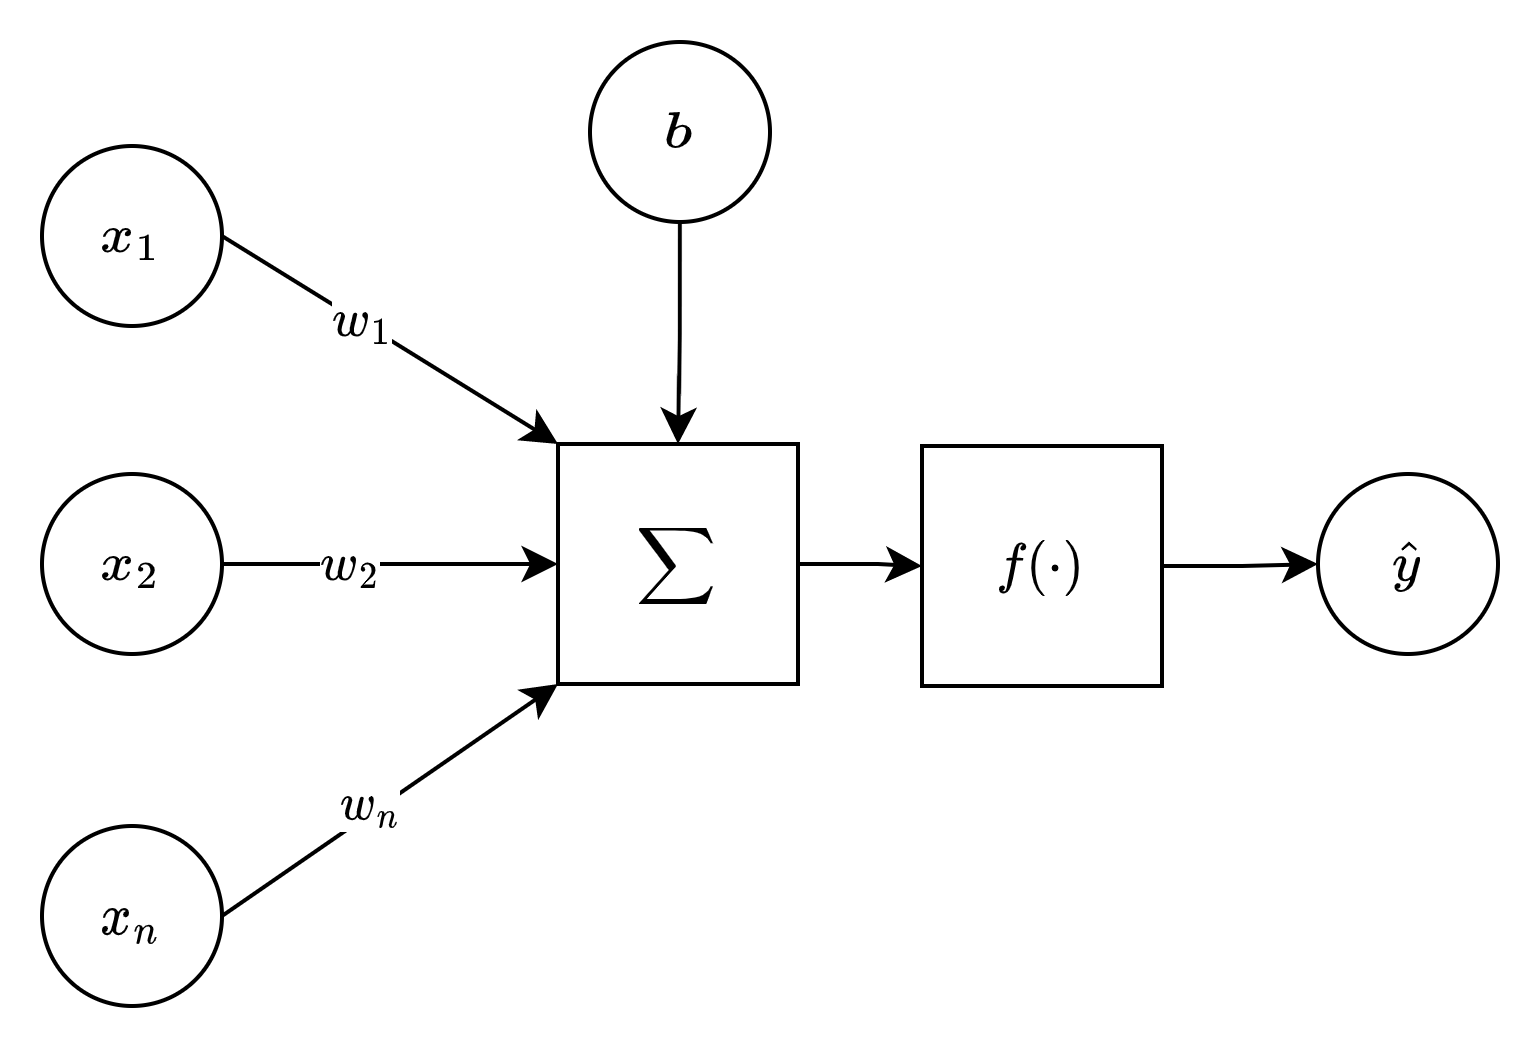
\includegraphics[width=1\linewidth]{figures/neuron_ai}
			\caption{Neurônio Artificial}
		\end{subfigure}
	\end{figure}
\end{frame}
%==========================================================================================
\begin{frame}
	\frametitle{Perceptron}
	\begin{itemize}
		\item Modelo mais básico de NN
		\item Um neurônio
		\item N entradas, Uma saída ŷ
	\end{itemize}
	\begin{figure}
		\centering
		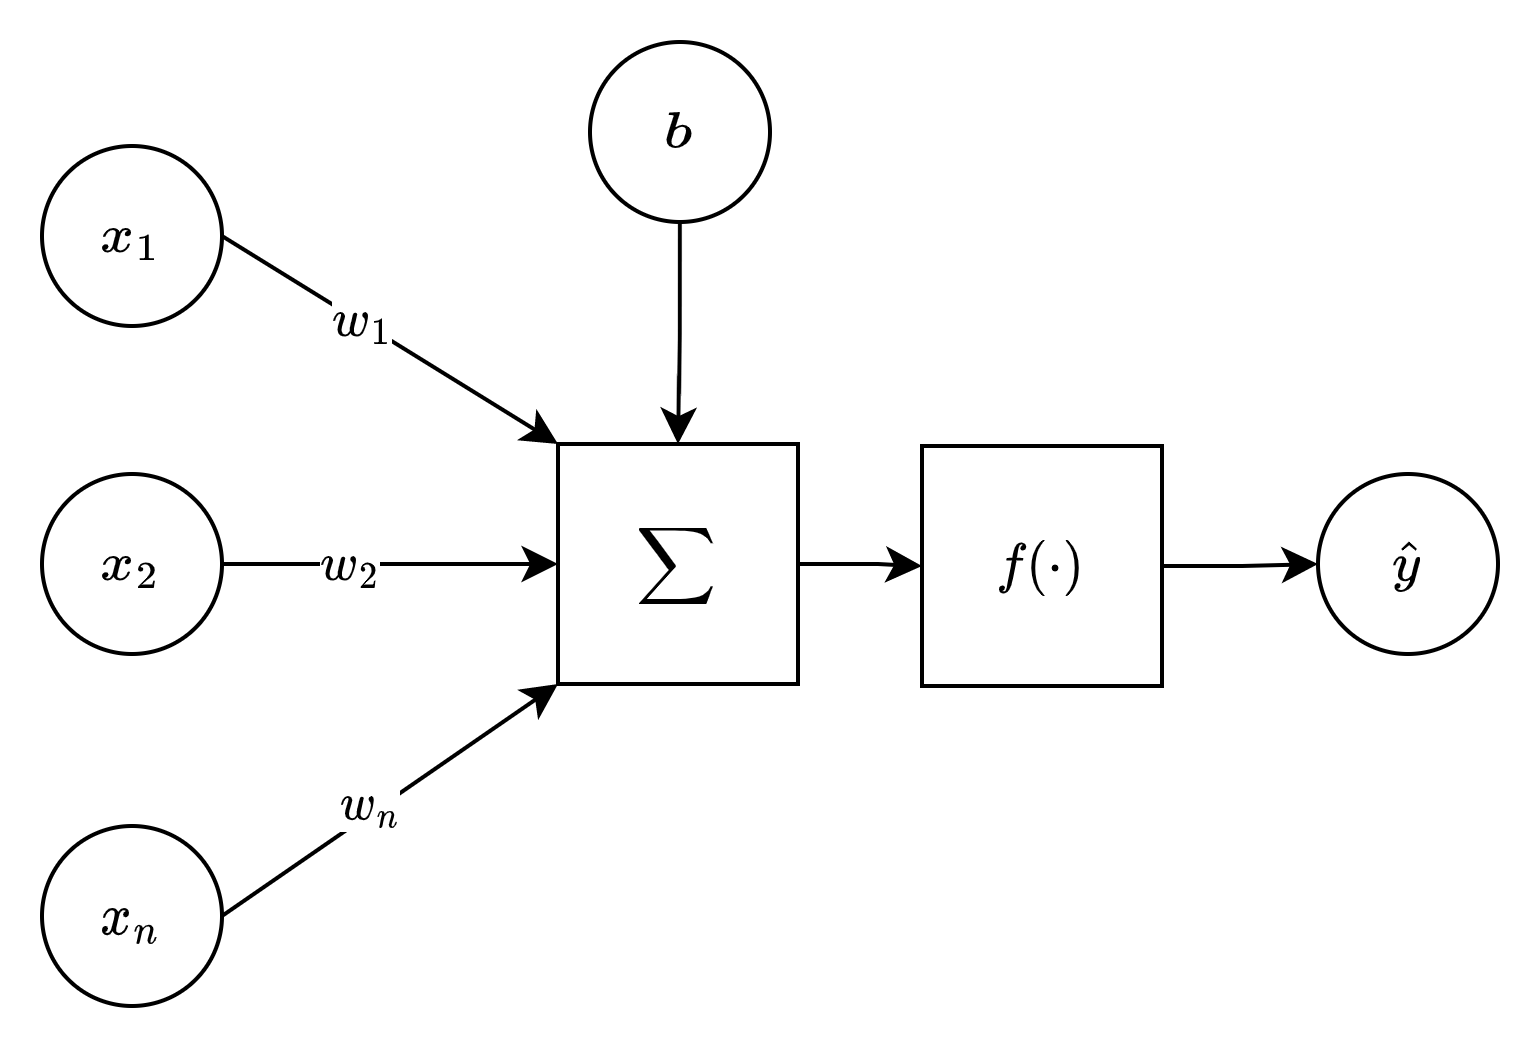
\includegraphics[width=0.4\linewidth]{figures/neuron_ai}
		\caption{Neurônio Artificial}
	\end{figure}

	\begin{gather*}
		\hat{y} = f( \sum_i w_i x_i + b)
	\end{gather*}
\end{frame}
%==========================================================================================
\begin{frame}
	\frametitle{Perceptron}
	\begin{block}{Função de ativação do perceptron}
		\begin{itemize}
			\item 0 se for negativo
			\item 1 se maior ou igual a 0
		\end{itemize}
	\end{block}
	
	\begin{figure}
		\centering
		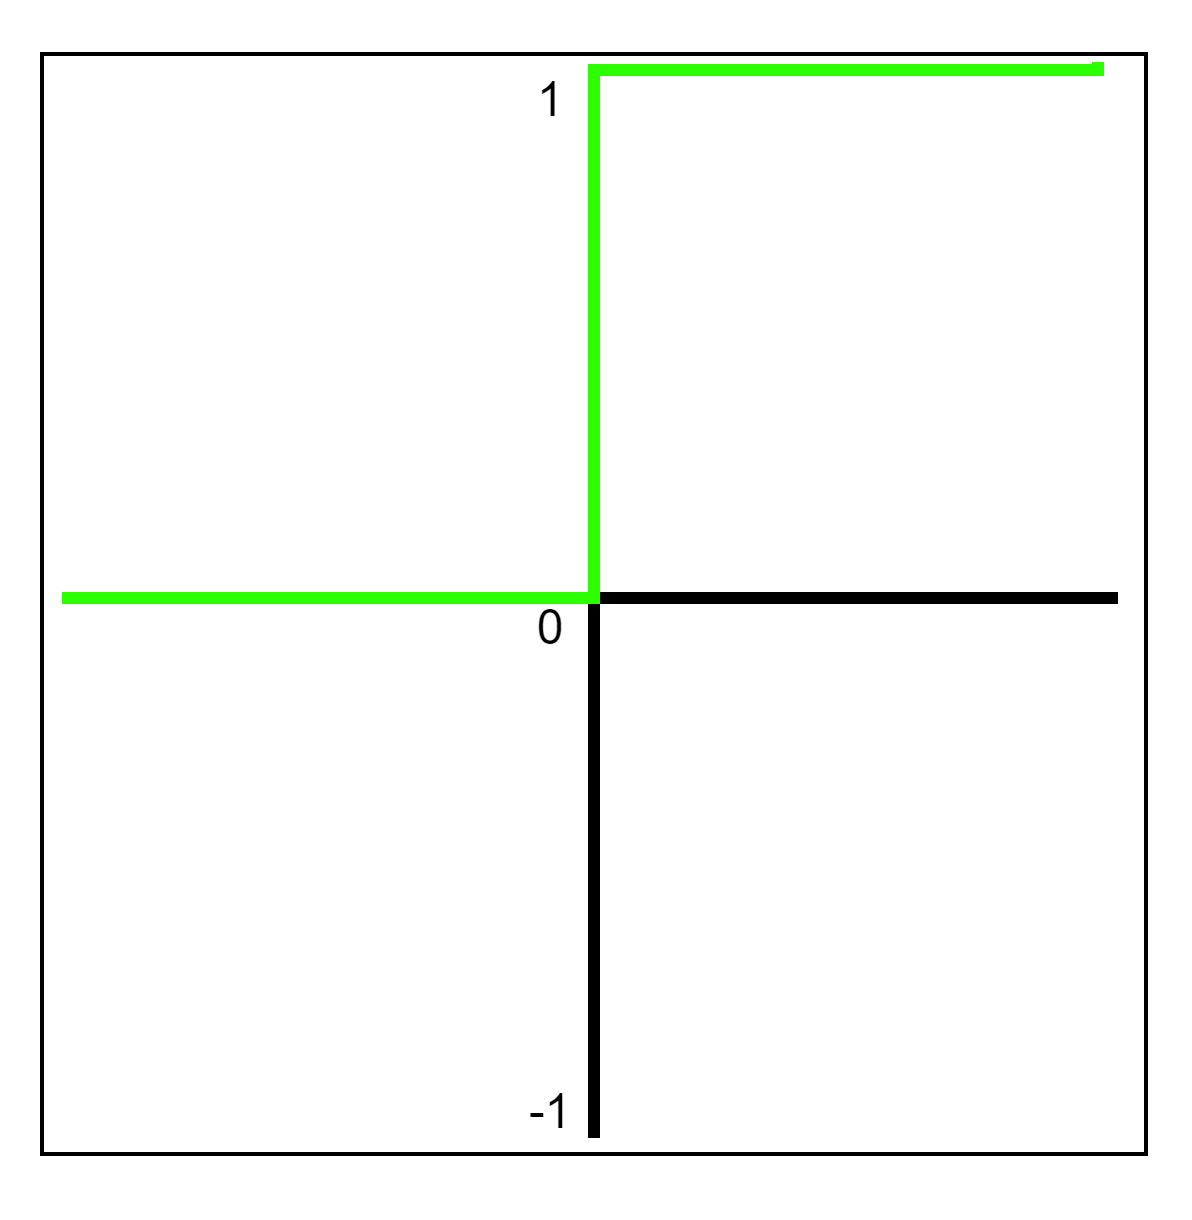
\includegraphics[width=0.4\linewidth]{figures/step_function}
	\end{figure}
\end{frame}
%==========================================================================================
\begin{frame}
	\frametitle{Perceptron}
	\begin{itemize}
		\item Modelo mais básico de NN
		\item Um neurônio
		\item N entradas, Uma saída ŷ
		\item Classificador binário linear
		\item Pode ser usado para Regressão
		\item Perceptron Rule
		\item Aprendizado Online
		\begin{itemize}
			\item Atualiza os pesos por amostra
		\end{itemize}
	\end{itemize}
	\begin{figure}
		\centering
		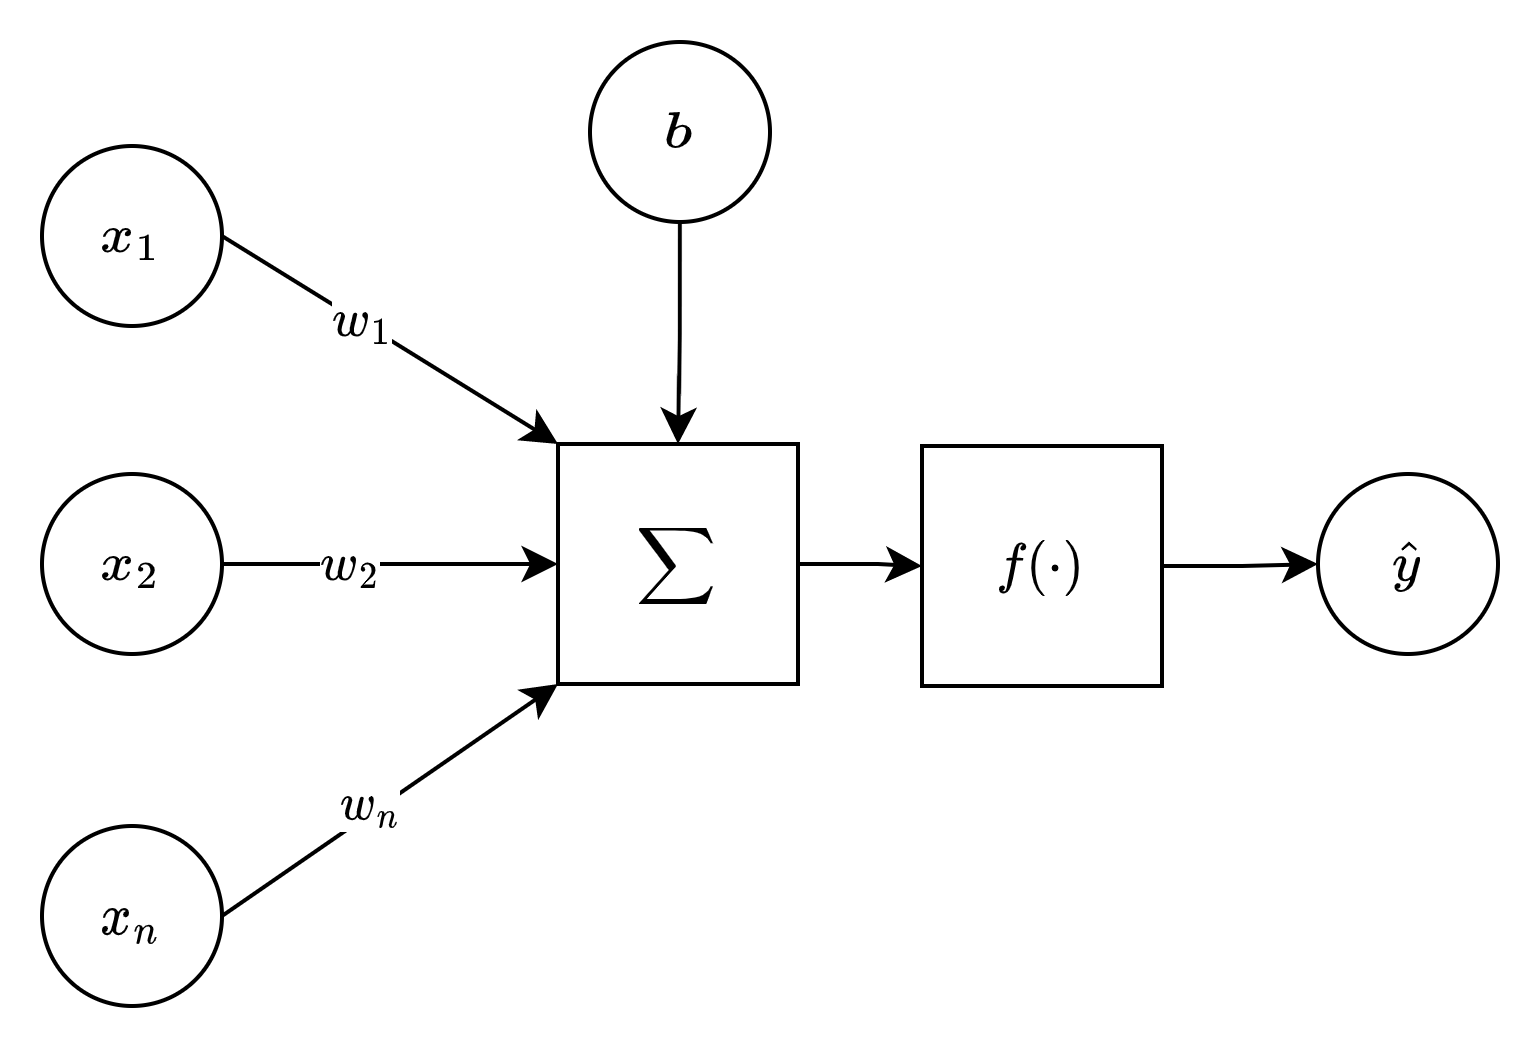
\includegraphics[width=0.4\linewidth]{figures/neuron_ai.png}
		\caption{Neurônio Artificial}
	\end{figure}
	
	\begin{gather*}
		\hat{y} = f( \sum_i w_i x_i + b)
	\end{gather*}
\end{frame}
%==========================================================================================
\begin{frame}
	\frametitle{Perceptron}
		\begin{block}{Perceptron Rule}
			O perceptron atualiza seus pesos utilizando a perceptron rule, não com o gradiente
	\end{block}
Atualização dos pesos:
	\begin{gather*}
		w_i = w_i + \lambda*(y_i -  \hat{y}_i)* x_i
	\end{gather*}
	Atualização do \textit{bias}:
	\begin{gather*}
		b_i = b_i + \lambda*(y_i -  \hat{y}_i)
	\end{gather*}
\begin{alertblock}{Observação importante}
``Quando a diferença yi -  ŷi for 0 então não ocorrerá a atualização dos pesos''
\end{alertblock}

\end{frame}
%==========================================================================================
\begin{frame}
	\frametitle{Perceptron}
	\begin{block}{Perceptron Rule}
		O perceptron atualiza seus pesos utilizando a perceptron rule, não com o gradiente
	\end{block}
	Atualização dos pesos:
	\begin{gather*}
		w_i = w_i + \lambda*(y_i -  \hat{y}_i)* x_i
	\end{gather*}
	Atualização do \textit{bias}:
	\begin{gather*}
		b_i = b_i + \lambda*(y_i -  \hat{y}_i)
	\end{gather*}

	
\end{frame}

%==========================================================================================
\begin{frame}
	\frametitle{Perceptron}
	\begin{block}{Ponto de partida diferente}
		Com diferentes pontos de partida, o algoritmo encontra quase a mesma solução, embora com diferentes taxas de convergência. Abaixo está uma ilustração do algoritmo GD para este problema:
		
		\href{https://github.com/mafaldasalomao/pavic_treinamento_ml/blob/main/Machine\%20Learning/figures/random_01.gif?raw=true}{\beamergotobutton{Caso 01}} \\
		\href{https://github.com/mafaldasalomao/pavic_treinamento_ml/blob/main/Machine\%20Learning/figures/random_02.gif?raw=true}{\beamergotobutton{Caso 02}}
	\end{block}
\end{frame}
%==========================================================================================
%==========================================================================================
%==========================================================================================
%==========================================================================================
%==========================================================================================
%==========================================================================================
%==========================================================================================
%==========================================================================================
%==========================================================================================
%==========================================================================================
%==========================================================================================
\section{Se Tornando Expert em Gradientes}

\begin{frame}
\frametitle{Highlighting text}

\begin{gather}
	W = np.random.randn(5, 10) \\
	X = np.random.randn(3, 10) \\
	Y = X.dot(W^{T}) \\
	f(x)
\end{gather}
%
%\begin{align}
%	a + b  q q= c \\        
%	a = c - b
%\end{align}
In this slide, some important text will be
\alert{highlighted} because it's important.
Please, don't abuse it.

\begin{block}{Remark}
Sample text
\end{block}

\begin{alertblock}{Important theorem}
Sample text in red box
\end{alertblock}

\begin{examples}
Sample text in green box. The title of the block is ``Examples".
\end{examples}
\end{frame}

\end{document}